\section{金属半导体的整流接触}
历史上,最早于20世纪初使用的第一个实用半导体器件其实就是金属--半导体二极管,这种二极管也被称为\uwave{点接触二极管}(Point Contact Diode),是通过将金属须接触裸露的半导体表面形成的。然而,这类金属--半导体二极管,形成难度大,可靠性也不好,因此在20世纪50年代左右被PN结取代。然而,随着半导体技术和真空技术的发展,稳定可靠的金属半导体结得以实现。在章首语中,我们已经提到过,金属--半导体结中的金半接触有两种类型
\begin{itemize}
    \item 高阻的整流接触(Rectifying Contact),此时金半接触具有类似PN结的整流特性。
    \item 低阻的欧姆接触(Ohmic Contact),此时金半接触具有很低的接触电阻,无附加影响。
\end{itemize}

在本节将先讨论金半整流接触,也就是\uwave{肖特基势垒二极管}(Schottky Barrier Diode)。

\subsection{金半整流接触的定性分析}
通常来说,整流接触都是由金属和N型半导体形成的,因此,本节我们会专注于这种情形。

\xref{fig:接触前}展示了金属和N型半导体接触前的能带图,其中,共同的真空能级$E_0$作为一个参考能级,代表了电子从金属或半导体表面逃逸所需达到的能量。除此之外,$e\phi_m$和$e\phi_s$则分别是金属和半导体中电子的\uwave{功函数}(Work Function),\empx{功函数表征了从费米能级至真空能级所需的能量}。不过,由于半导体的费米能级位于禁带中,在费米能级处并不存在电子,功函数没有实际意义,故半导体中更常用的是以$e\chi$表示的\uwave{电子亲合能}(Electron Affinity),\empx{电子亲合能表征了从导带底至真空能级所需的能量}。而功函数与电子亲合能的差$\phi_s-\chi$则记为$\phi_n$。

\begin{Figure}[金半整流接触的能带图]
    \begin{FigureSub}[接触前]
        \includegraphics[scale=0.8]{build/Chapter03A_01.fig.pdf}
    \end{FigureSub}
    \hspace{0.5cm}
    \begin{FigureSub}[接触后]
        \includegraphics[scale=0.8]{build/Chapter03A_02.fig.pdf}
    \end{FigureSub}
\end{Figure}

这里需要说明的是电势量的命名规律,通常以费米能级$E_F$为下界的电势量均会以$\phi$命名,包括$\phi_m,\phi_s,\phi_n$和后面的$\phi_{B0}$等,而其他的电势量则用其他的名称,包括$\chi$和后面的$V_{bi}$等。

\begin{BoxDefinition}[金属的功函数]
    金属的功函数$e\phi_m$,定义为费米能级至真空能级所需的能量
    \begin{Equation}
        e\phi_m=E_0-E_F
    \end{Equation}
\end{BoxDefinition}

\begin{BoxDefinition}[半导体的功函数]*
    半导体的功函数$e\phi_s$,定义为费米能级至真空能级所需的能量
    \begin{Equation}
        e\phi_s=E_0-E_F
    \end{Equation}
    半导体的电子亲和能$e\chi$,定义为导带底至真空能级所需的能量
    \begin{Equation}
        e\chi=E_0-E_c
    \end{Equation}
    而两者的差$\phi_s-\chi$则定义为$\phi_n$,其中$e\phi_n$代表导带底和费米能级的能量差
    \begin{Equation}
        \phi_n=\phi_s-\chi\qquad e\phi_n=E_c-E_F
    \end{Equation}
\end{BoxDefinition}

在\xref{tab:部分金属的功函数}和\xref{tab:部分半导体的电子亲合能}中,列出了部分金属的$\phi_m$和部分半导体的$\chi$。

\begin{Tablex}[部分金属的功函数]{XX}
<金属&金属的功函数$\phi_m$\\>
银\xce{Ag}&4.26\\ 
铝\xce{Al}&4.28\\ 
金\xce{Au}&5.1\\ 
铬\xce{Cr}&4.5\\ 
钼\xce{Mo}&4.6\\ 
镍\xce{Ni}&5.15\\ 
钯\xce{Pd}&5.12\\ 
铂\xce{Pt}&5.65\\ 
钛\xce{Ti}&4.33\\ 
钨\xce{W}&4.55\\ 
\end{Tablex}

\begin{Tablex}[部分半导体的电子亲合能]{XX}
<半导体&半导体的电子亲合能$\chi$\\>
锗\xce{Ge}&4.13\\
硅\xce{Si}&4.01\\
砷化镓\xce{GaAs}&4.07\\
砷化铝\xce{AlAs}&3.5\\
\end{Tablex}

值得注意的是,在\xref{fig:接触前}中,我们假定了$\phi_m>\phi_s$,即,金属的功函数高于半导体的功函数,或者说,金属的费米能级比半导体低。实际上,$\phi_m$和$\phi_s$的关系将决定金半接触的类型
\begin{itemize}
    \item 若$\phi_m>\phi_s$,半导体费米能级较高,产生整流接触(接触后能带向上弯曲)。
    \item 若$\phi_m<\phi_s$,半导体费米能级较低,产生欧姆接触(接触后能带向下弯曲)。
\end{itemize}
由于本节考虑整流接触,故本节总是默认$\phi_m>\phi_s$成立。

\xref{fig:接触后}展示了金属和N型半导体接触后的能带图,由于接触前,半导体的费米能级在金属之上,为了使系统具有统一的常量,两者接触后,半导体表面附近的电子将流入能量更低的金属中,半导体表面的能带将向上弯曲,带正电的施主原子留在半导体中,形成空间电荷区。

\begin{BoxDefinition}[金半接触的肖特基势垒]
    金半接触时,\uwave{肖特基势垒}(Schottky Barrier)是指电子从金属进入半导体所需的能量
    \begin{Equation}
        e\phi_{B0}=(E_{c})_\te{边界}-E_F
    \end{Equation}
    或者可以表示为
    \begin{Equation}
        \phi_{B0}=\phi_m-\chi
    \end{Equation}
\end{BoxDefinition}

\begin{BoxDefinition}[金半接触的内建电势差]
    金半接触时,内建电势差是指电子从半导体进入金属所需的能量
    \begin{Equation}
        eV_{bi}=(E_c)_\te{边界}-E_c
    \end{Equation}
    或者可以表示为
    \begin{Equation}
        V_{bi}=\phi_m-\chi-\phi_n=\phi_{B0}-\phi_n
    \end{Equation}
\end{BoxDefinition}

简单来说,金半接触时
\begin{itemize}
    \item 电子从金属进入半导体的势垒,称为肖特基势垒,以$\phi_{B0}$或$e\phi_{B0}$表示。
    \item 电子从半导体进入金属的势垒,称为内建电势差,以$V_{bi}$或$eV_{bi}$表示,类似PN结的。
\end{itemize}

现在我们已经比较清楚金半整流接触的能带图了,那么当外加偏置电压时,金半整流接触的能带图将如何变化呢?首先要弄清的是,金半接触时“正向”和“反向”是如何定义的,在整流接触中,金属为正极,N型半导体为负极,换言之,金属取代了PN结的P型半导体。事实是,当外加电压时,外加电压完全落在半导体侧势垒上,金属侧势垒将保持$\phi_{B0}$不变



\begin{itemize}
    \item 当外加正向电压$V_a$时,由于半导体侧势垒由$V_{bi}$降低至$V_{bi}-V_a$,半导体至金属的电子运动更容易了,半导体至金属的电子流将占优势,形成正向电流。同时,由于越大的正向电压意味着半导体侧势垒降低的越多,\empx{正向电流会随正向电压的增大而指数级增大}。
    \item 当外加反向电压$V_R$时,由于半导体侧势垒由$V_{bi}$升高至$V_{bi}+V_R$,这将导致半导体至金属的电子流逐渐减小至零,此时,金属至半导体的电子流将占优势,形成反向电流。反向电流的的大小取决于金属侧势垒$\phi_{B0}$的高度,但由于金属侧势垒$\phi_{B0}$不随外加电压变化,金属至半导体的电流是恒定的,换言之,\empx{反向电流将随反向电压增大趋于定值}。
\end{itemize}

由此可见,金属半导体的整流接触具有与PN结相似的整流特性。

\begin{Table}[金半整流接触外加偏置电压时的能带变化]{|c|c|c|}
    \xcell<c>[1em][0em]
    {\includegraphics[width=4.5cm]{build/Chapter03A_03.fig.pdf}}&
    \xcell<c>[1em][0em]
    {\includegraphics[width=4.5cm]{build/Chapter03A_05.fig.pdf}}&
    \xcell<c>[1em][0em]
    {\includegraphics[width=4.5cm]{build/Chapter03A_04.fig.pdf}}\\
    零偏&正偏(正向电压$V_a$)&反偏(反向电压$V_R$)\\
\end{Table}

\subsection{金半整流接触的理想静电特性}
金半整流接触和PN结是类似的,两者均有均匀掺杂且适用突变近似的空间电荷区,因此,金半接触包括“电场分布、电场分布、空间电荷区宽度、势垒电容”在内的静电特性都可以直接从PN结的相关结论中得来(\xref{fml:空间电荷区的电场}、\xref{fml:空间电荷区的电势}、\xref{fml:反偏时的空间电荷区宽度}、\xref{fml:二极管的势垒电容}),唯一的一项差异在于,金半接触的空间电荷区仅分布在N型半导体,金属中没有空间电荷区,故,金半接触相当于P$^{+}$N结,适用$x_n\gg x_p, W=x_n$以及$N_d\ll N_a$即$N_aN_d/(N_a+N_d)=N_d$的近似。

\begin{BoxFormula}[金半整流接触的电场分布]
    金半接触的电场分布满足
    \begin{Equation}
        \E(x)=-\frac{eN_d}{\epsilon_s}(x_n-x)
    \end{Equation}
\end{BoxFormula}

\begin{BoxFormula}[金半整流接触的电势分布]
    金半接触的电势分布满足
    \begin{Equation}
        \phi(x)=V_{bi}-\frac{eN_d}{2\epsilon_s}(x_n-x)^2
    \end{Equation}
\end{BoxFormula}

\begin{BoxFormula}[金半整流接触的空间电荷区宽度]
    金半整流接触的空间电荷区宽度满足
    \begin{Equation}
        W=x_n=\qty[\frac{2\epsilon_s(V_{bi}+V_R)}{eN_d}]^{1/2}
    \end{Equation}
\end{BoxFormula}

\begin{BoxFormula}[金半整流接触的势垒电容]
    金半整流接触的势垒电容满足
    \begin{Equation}
        C_j=A\qty[\frac{e\epsilon_sN_d}{2(V_{bi}+V_R)}]^{1/2}
    \end{Equation}
\end{BoxFormula}

\subsection{影响势垒高度的非理想因素}

有一些非理想因素会影响肖特基势垒的高度,包括镜像力和表面态。

\subsubsection{镜像力}
金属具有静电感应的特性,当电子在空间电荷区中运动时,除了受到空间电荷区中电荷的吸引外,还会在金属表面感应出正电荷。空间电荷区的电势我们在\xref{subsec:金半整流接触的理想静电特性}已经用泊松方程计算出来了,然而,金属表面感应正电荷产生的电势却尚没有纳入考虑。但问题在于,金属表面的电荷对电子的吸引该如何计算呢,这是比较复杂的。不过所幸的是,有一些简单的办法可以 解决这个问题。\uwave{镜像法}(Method of Images)指出\cite{wiki:镜像法},\empx{金属表面的感应电荷对点电荷的吸引力,等同于将金属视为一面镜子,镜子中点电荷的镜像电荷对点电荷的吸引力}。换言之,若我们要分析金属表面的感应电荷对电子的吸引,只要假象金属是一面镜子,镜子中有一个电子的\uwave{镜像电荷}(Image Charge),即一个位置上镜面对称但电荷相反(带正电)的点电荷,并考虑镜像电荷对电子的\uwave{镜像力}(Image Force),由此就将表面电荷的作用转换为点电荷的作用。

那么,镜像力将对金半整流接触的势垒发生什么影响呢?
\begin{BoxFormula}[镜像力的势垒降低]
    镜像力将使金半整流接触的势垒高度降低,且势垒的最高点向半导体侧内移。

    势垒的降低量为(对于电势而言是增加量)
    \begin{Equation}
        \delt{\phi}=\frac{1}{4}\sqrt[\uproot{16}\leftroot{-2}4]{\frac{2e^3N_d(V_{bi}+V_R)}{\pi^2\epsilon_s^3}}
    \end{Equation}
    势垒的最高点内偏,现在位于(原先位于$x=0$处)
    \begin{Equation}
        x_{m}=\frac{1}{4(\pi N_dx_d)^{1/2}}
    \end{Equation}
\end{BoxFormula}

\begin{Proof}
    设电子位于$x$处,那么镜像电荷将位于$-x$处,依照库伦作用,吸引力为
    \begin{Equation}&[1]
        F=-\frac{1}{4\pi\epsilon_s}\frac{e^2}{(2x)^2}=-\frac{e^2}{16\pi\epsilon_s}\frac{1}{x^2}
    \end{Equation}
    而另外一方面,电场力和电场的关系是
    \begin{Equation}&[2]
        F=-eE
    \end{Equation}
    镜像电荷产生的电场$\E_M(x)$就为
    \begin{Equation}&[3]
        \E_M(x)=\frac{e}{16\pi\epsilon_s}\frac{1}{x^2}
    \end{Equation}
    镜像电荷产生的电势$\phi_M(x)$可通过对$\E_M(x)$积分得到
    \begin{Equation}&[4]
        \phi_M(x)=-\Int\E(x)\dx=\frac{e}{16\pi\epsilon_s}\Int\frac{1}{x^2}\dx=\frac{e}{16\pi\epsilon_s}\frac{1}{x}+C
    \end{Equation}
    此处定$\phi_M(x)$在无穷远处的电势为零,故
    \begin{Equation}&[5]
        \phi_M(x)=\frac{e}{16\pi\epsilon_s}\frac{1}{x}
    \end{Equation}
    原先的电势改记为$\phi_0(x)$,根据\fancyref{fml:金半整流接触的电势分布}
    \begin{Equation}&[6]
        \phi_0(x)=\begin{cases}
            \mal{V_{bi}-\frac{eN_d}{2\epsilon_s}(x_n-x)^2}, &0<x<x_n\\
            \mal{V_{bi}}, &x\geq x_n
        \end{cases}
    \end{Equation}
    将\xrefpeq{5}和\xrefpeq{6}相加,得到总电势$\phi(x)$
    \begin{Equation}&[7]
        \phi(x)=\phi_0(x)+\phi_M(x)=\begin{cases}
            \mal{V_{bi}+\frac{e}{16\pi\epsilon_s}\frac{1}{x}-\frac{eN_d}{2\epsilon_s}(x_n-x)^2}, &0<x<x_n\\[5mm]
            \mal{V_{bi}+\frac{e}{16\pi\epsilon_s}\frac{1}{x}}, &x\geq x_n
        \end{cases}
        \hspace{-0.2cm}
    \end{Equation}
    原先的电场改记为$\E_0(x)$,根据\fancyref{fml:金半整流接触的电场分布}
    \begin{Equation}&[8]
        \E_0(x)=-\frac{eN_d}{\epsilon_s}(x_n-x)
    \end{Equation}
    镜像电荷的电场$\E_M(x)$已经在\xrefpeq{3}中求出来了
    \begin{Equation}&[9]
        \E_M(x)=\frac{e}{16\pi\epsilon_s}\frac{1}{x^2}
    \end{Equation}
    镜像电荷对电势的影响,关键在于求出\xrefpeq{7}中电势函数$\phi(x)$的极小值的出现位置$x_m$和极小电势$\delt{\phi}$(这里$\delt{\phi}$是相较$\phi_0(x)$的极小值点而言的,而$\phi_0(x)$的极小值为零),我们愿意相信$x_m\ll x_n$,因此,确定电势的极小值点的位置$x_m$,只需要分析电场$\E_0(x), \E_M(x)$在何处相等即可,因此,我们联立\xrefpeq{8}和\xrefpeq{9},构成方程$\E_0(x_m)=\E_M(x_m)$
    \begin{Equation}&[10]
        \frac{e}{16\pi\epsilon_s}\frac{1}{x_m^2}=-\frac{eN_d}{\epsilon_s}(x_n-x_m)
    \end{Equation}
    这是一个关于$x_m$的三次方程,并不好解,援引$x_m\ll x_n$的近似
    \begin{Equation}&[11]
        \frac{e}{16\pi\epsilon_s}\frac{1}{x_m^2}=-\frac{eN_d}{\epsilon_s}x_n
    \end{Equation}
    容易得出
    \begin{Equation}&[12]
        x_m^2=\frac{1}{16\pi N_dx_n}
    \end{Equation}
    即
    \begin{Equation}&[13]
        x_m=\frac{1}{4(\pi N_dx_n)^{1/2}}
    \end{Equation}
    现在代入计算$\delt{\phi}=\phi(x_m)$,由于我们确信$x_m\ll x_n$,故\xrefpeq{7}的$\phi(x)$可以仅取第一部分
    \begin{Equation}&[14]
        \phi(x)=V_{bi}+\frac{e}{16\pi\epsilon_s}\frac{1}{x}-\frac{eN_d}{2\epsilon_s}(x_n-x)^2
    \end{Equation}
    但为了简化结果,这里代入时忽略$\phi(x)$有关镜像力的项,即回归$\phi_0(x)$
    \begin{Equation}&[15]
        \phi(x)=V_{bi}-\frac{eN_d}{2\epsilon_s}(x_n-x)^2
    \end{Equation}
    这就得到
    \begin{Equation}&[16]
        \delt{\phi}=V_{bi}-\frac{eN_d}{2\epsilon_s}(x_n-x_m)^2
    \end{Equation}
    展开
    \begin{Equation}&[17]
        \delt{\phi}=V_{bi}-\frac{eN_d}{2\epsilon_s}(x_n^2-2xnx_m+x_m^2)
    \end{Equation}
    依据\fancyref{fml:空间电荷区的电势}
    \begin{Equation}&[18]
        V_{bi}=\frac{e}{2\epsilon_s}x_n^2
    \end{Equation}
    运用\xrefpeq{18}就可以将\xrefpeq{17}简化为
    \begin{Equation}&[19]
        \delt{\phi}=\frac{eN_d}{2\epsilon_s}\qty(2x_nx_m-x_m^2)
    \end{Equation}
    运用$x_m\ll x_n$忽略二次项$x_m^2$
    \begin{Equation}
        \delt{\phi}=\frac{eN_d}{\epsilon_s}x_nx_m
    \end{Equation}
    代入\xrefpeq{13}给出的$x_m$
    \begin{Equation}
        \delt{\phi}=\frac{1}{4}\frac{eN_d}{\epsilon_s}x_n\sqrt{\frac{1}{\pi N_dx_n}}
    \end{Equation}
    将各项整合到根号下
    \begin{Equation}
        \delt{\phi}=\frac{1}{4}\sqrt{\frac{e^2N_dx_n}{\pi\epsilon_s^2}}
    \end{Equation}
    有趣的是我们还可以将$x_n$代入,根据\fancyref{fml:金半整流接触的空间电荷区宽度}
    \begin{Equation}
        \delt{\phi}=\frac{1}{4}\sqrt{\frac{e^2N_d}{\pi\epsilon_s^2}\sqrt{\frac{2\epsilon_s(V_{bi}+V_R)}{eN_d}}}
    \end{Equation}
    将各项整合到内层根号,并合并内外层根号
    \begin{Equation}
        \delt{\phi}=\sqrt[\uproot{16}\leftroot{-2}4]{\frac{2e^4N_d(V_{bi}+V_R)}{\pi^2\epsilon_s^3}}
    \end{Equation}
    至此,我们就完成了所有的计算。
\end{Proof}

镜像力对电势曲线的影响如\xref{fig:镜像力对电势曲线的影响}所示,其中标注了$\delt{\phi}$和实际近似计算的$\delt{\phi}$的位置。

\begin{Figure}[镜像力对电势曲线的影响]
    \includegraphics{build/Chapter03A_06.fig.pdf}
\end{Figure}

镜像力的影响反映在能带图上的效果如\xref{tab:镜像力对势垒的影响}所示,其实际就是将\xref{fig:镜像力对电势曲线的影响}上下颠倒了一下(电势能与电势相差$-e$倍)。由\xref{tab:镜像力对势垒的影响}可以看出,
\empx{镜像力削弱了势垒并使势垒向半导体侧发生偏移}。

\begin{Table}[镜像力对势垒的影响]{|c|c|}
    \xcell<c>[1em][0em]
    {\includegraphics[width=4.5cm]{build/Chapter03A_03.fig.pdf}}&
    \xcell<c>[1em][0em]
    {\includegraphics[width=4.5cm]{build/Chapter03A_07.fig.pdf}}\\
    理想状态&镜像力的影响\\
\end{Table}

镜像力对电势的影响$\delt{\phi}$其实还是比较微弱的,随着反向电压$V_R$的增大缓慢增大。

\subsubsection{表面态}
金属和半导体接触时,如\xref{tab:表面态对势垒的影响}所示,两者实际上并不是紧密接触的,金属和半导体间存在一层很薄的绝缘\uwave{界面层}(Interfacial Layer)。界面层并不影响金属和半导体间的电子流动,但可以在金属和半导体间维持一定的电势差$\delt{V_\te{ox}}$,表现为半导体的真空能级将低于金属,而我们从图中可以看出,半导体真空能级的降低使得能带的弯曲也减弱了,换言之,势垒降低了。

那么,为何界面层会导致电势差$\delt{V_\te{ox}}$?这是因为半导体会在界面层处形成\uwave{表面态}(Surface States)的分布,表面态均位于禁带中。表面态存在两类,分别是施主表面态和受主表面态
\begin{itemize}
    \item 施主表面态(类似N区产生电子的施主原子),有电子时为中性,无电子时带正电。
    \item 受主表面态(类似P区产生空穴的受主原子),无电子时为中性,有电子时带负电。
\end{itemize}
简单起见,我们可以假定禁带存在这样一个电势$\phi_0$(这里$e\phi_0$是相对边界处价带顶$E_v$而言的)的分界线,在$e\phi_0$以下的表面态均为施主态,在$e\phi_0$以上的表面态均为受主态。我们知道,若需要使表面态呈中性,施主态内需有电子,受主态需为空,通常来说$e\phi_0$位于禁带下三分之一的位置,而N型半导体的费米能级$E_F$往往比较靠近导带,因此$E_F$将高于$e\phi_0$,那么$E_F$和$e\phi_0$间的表面受主态就将存在电子,使半导体表面带负电。这就是$\delt{V_\te{ox}}$的来源。

很明显,对于一定的$\delt{V_\te{ox}}$半导体表面所需的负电荷$Q_{SS}$是一定的,而$Q_{SS}$受到两个因素决定,其一是$E_F$与$e\phi_0$的间距,该间距内的表面态将带负电,其二是表面态的密度$D_{it}$,很明显$Q_{SS}$正比于两者的乘积。因此,若密度$D_{it}$越大,间距就可以越小。问题是,间距是由谁控制的呢?尽管$e\phi_0$是固定的,但是$e\phi_0$是相对表面处价带顶而言的,而表面处能带是可以向上弯曲的,弯曲的少些间距就大些,弯曲的多些间距就小些。极限情况是,态密度$D_{it}$无穷大,此时能带就会弯曲使$e\phi_0$和$E_F$间距刚好为零,换言之,此时$e\phi_0$就落在$E_F$上。这种情况下的,肖特基势垒$\phi_{Bn}$就不再由金属和半导体本身的性质\footnote{理想状态下的肖特基势垒记为$\phi_{B0}$,而考虑镜像力和表面态这些非理想因素后,就改记为$\phi_{Bn}$},即$\phi_{Bn}=\phi_m-\chi$确定了,而是完全由表面态的性质,即$\phi_{Bn}=E_g/e-\phi_0$确定了,与功函数$\phi_m$和电子亲合能$\chi$无关。

\begin{Table}[表面态对势垒的影响]{|c|c|}
    \xcell<c>[1em][0em]
    {\includegraphics[scale=0.8]{build/Chapter03A_09.fig.pdf}}&
    \xcell<c>[1em][0em]
    {\includegraphics[scale=0.8]{build/Chapter03A_08.fig.pdf}}\\
    理想状态&表面态的影响\\
\end{Table}

由此可见,金半接触时,接触表面的状态将对金半接触的性质产生很大的影响。

这里也可以做一些定量的分析,有公式指出以下的参数的关系
\begin{Equation}
    (E_g-e\phi_0-e\phi_{Bn})=\frac{1}{eD_\te{it}}\sqrt{2e\epsilon_sN_d(\phi_{Bn}-\phi_n)}-\frac{\epsilon_i}{eD_\te{it}\delta}[\phi_m-(\chi+\phi_{Bn})]
\end{Equation}
1. 第一种情况,若$D_\te{it}\to\infty$,则右侧两项均可以忽略,有
\begin{Equation}
    \phi_{Bn}=E_g/e-\phi_0
\end{Equation}
这种情况下,势垒高度完全由禁带宽度$E_g$和$\phi_0$确定,势垒高度与金属功函数$\phi_m$和半导体的电子亲合能$\chi$无关。费米能级$E_F$被钉在了表面势$e\phi_0$上,该现象称为\uwave{钉扎}(Pinning)。

2. 第二种情况,若$D_\te{it}\delta\to 0$,则只需考虑右侧第二项,有
\begin{Equation}
    \phi_{Bn}=(\phi_m-\chi)
\end{Equation}
这就回到了最初考虑的理想情况,即\fancyref{def:金半接触的肖特基势垒}。

\subsection{金半整流接触的电流电压关系}
金半结和PN结的电流传输运机构有所不同,金半结是多子导电,PN结是少子导电。金半整流接触的基本过程是电子运动通过势垒,取决于势垒的情况,有两种不同的理论来解释
\begin{itemize}
    \item 当势垒较薄时,应使用\uwave{热电子发射理论}(Thermionic Emission Theory)。
    \item 当势垒较厚时,应使用\uwave{扩散理论}(Diffusion Theory)。\footnote{这里的势垒较薄或较厚,是相对于电子的平均自由程而言的。}
\end{itemize}

在此,我们主要讨论热电子发射理论。热电子发射理论的观点是,由于势垒很薄,此时,势垒的形状不重要,势垒的高度将起决定性作用。半导体内部的电子只要有足够的能量超越势垒的顶点,就可以通过半导体进入金属。故电流的计算,就归结为计算超越势垒的载流子数目。


\begin{BoxFormula}[金半结的电流--电压关系]
    金属半导体整流接触的电流--电压关系,依照热电子发射理论为
    \begin{Equation}
        J=J_{sT}\qty[\exp(\frac{eV_a}{\kB T})-1]
    \end{Equation}
    其中$J_{sT}$为
    \begin{Equation}
        J_{sT}=A^{*}T^2\exp\qty(-\frac{e\phi_{Bn}}{\kB T})
    \end{Equation}
    其中$A^{*}$称为\uwave{有效理查逊常数}(Effective Richardson Constant)
    \begin{Equation}
        A^{*}=\frac{em_{n}^{*}\kB^2}{2\pi^2\hbar^3}
    \end{Equation}
\end{BoxFormula}

\begin{Proof}
    假定势垒高度$eV_{bi}\gg\kB T$。由于通过势垒交换的电子数,只占了半导体中总电子数的很小一部分,半导体内的电子浓度可以视为无关电流大小的常数,这样问题就变得容易处理些了。
    
    根据半导体物理的知识,单位体积中能量在$E$至$E+\dd{E}$间的电子数为
    \begin{Equation}&[1]
        \qquad\qquad\qquad
        \dd{n}=\frac{1}{V}g_{c}(E)f(E)\dd{E}=
        \frac{(2\mne)^{3/2}}{2\pi^2\hbar^3}
        (E-E_{c})^{1/2}
        \exp(\frac{E_{F}-E}{\kB T})\dd{E}
        \qquad\qquad\qquad
    \end{Equation}
    稍作转化
    \begin{Equation}&[2]
        \dd{n}=\frac{(2\mne)^{3/2}}{2\pi^2\hbar^3}
        (E-E_{c})^{1/2}
        \exp(\frac{E_{F}-E_{c}}{\kB T})
        \exp(\frac{E_{c}-E}{\kB T})\dd{E}
    \end{Equation}
    设$v$为电子运动的速度,那么
    \begin{Equation}&[3]
        E-E_{c}=\frac{1}{2}\mne v^2\qquad
        \dd{E}=\mne v\dd{v}
    \end{Equation}
    将\xrefpeq{3}代入\xrefpeq{2}
    \begin{Equation}&[4]
        \qquad\qquad
        \dd{n}=\frac{(2\mne)^{3/2}}{2\pi^2\hbar^3}
        \qty(\frac{1}{2}\mne v^2)^{1/2}
        \exp(\frac{E_{F}-E_{c}}{\kB T})
        \exp(-\frac{\mne v^2}{2\kB T})
        \mne v\dd{v}
        \qquad\qquad
    \end{Equation}
    整理
    \begin{Equation}&[5]
        \dd{n}=
        \frac{(\mne)^3}{\pi^2\hbar^3}
        \exp(\frac{E_{F}-E_{c}}{\kB T})
        \exp(-\frac{\mne v^2}{2\kB T})v^2\dd{v}
    \end{Equation}
    凑系数
    \begin{Equation}&[6]
        \qquad\quad
        \dd{n}=
        4\pi\qty(\frac{\mne}{2\pi\kB T})^{3/2}
        \qty[
            2\qty(\frac{\mne\kB T}{2\pi\hbar^2})^{3/2}
            \exp(\frac{E_{F}-E_{c}}{\kB T})
        ]\exp(-\frac{\mne v^2}{2\kB T})v^2\dd{v}
        \qquad\quad
    \end{Equation}
    而我们知道
    \begin{Equation}&[7]
        n_0=N_{c}\exp(\frac{E_{F}-E_{c}}{\kB T})\qquad N_{c}=2\qty(\frac{\mne\kB T}{2\pi\hbar^2})^{3/2}
    \end{Equation}
    将\xrefpeq{7}代入\xrefpeq{6}
    \begin{Equation}&[8]
        \dd{n}=
        4\pi n_0\qty(\frac{\mne}{2\pi\kB T})^{3/2}
        v^2\exp(-\frac{\mne v^2}{2\kB T})\dd{v}
    \end{Equation}
    这里$\dd{n}$表示单位体积重速度在$v$至$v+\dd{v}$间的电子数。

    这是一维的情况,容易推广至三维,注意$4\pi v^2$消失了,它们被作为球坐标的系数了
    \begin{Equation}&[9]
        \dd{n}=n_0\qty(\frac{\mne}{2\pi\kB T})^{3/2}
        \exp[-\frac{\mne(v_x^2+v_y^2+v_z^2)}{2\kB T}]\dd{v_x}\dd{v_y}\dd{v_z}
    \end{Equation}
    那么,有多少电子可以在单位时间内到达金属和半导体的界面呢?设半导体指向金属的方向为$v_x$的正方向,很明显,速度在$v_x$至$v_x+\dd{v_x}$间的电子,只要在距离界面$v_x$距离内,就都可以到达界面。因此,就单位截面积,能到达界面的电子数目是(即体积$v_x$中的电子数)
    \begin{Equation}&[10]
        \qquad\qquad
        \dd{N}=v_x\dd{n}=n_0\qty(\frac{\mne}{2\pi\kB T})^{3/2}
        \exp[-\frac{\mne(v_x^2+v_y^2+v_z^2)}{2\kB T}]v_x\dd{v_x}\dd{v_y}\dd{v_z}
        \qquad\qquad
    \end{Equation}
    而到达界面的电子,要越过势垒,必须满足
    \begin{Equation}&[11]
        \frac{1}{2}\mne v_x^2\geq e(V_{bi}-V)
    \end{Equation}
    即所需的$v_x$方向的最小速度是
    \begin{Equation}&[12]
        v_{x0}=\sqrt{\frac{2e(V_{bi}-V)}{\mne}}
    \end{Equation}
    而$v_y,v_z$方向的速度则没有任何的限制。

    因此,从半导体流向金属的电子流所形成的电流密度就是
    \begin{Equation}&[13]
        \qquad
        J_{{s}\to{m}}=
        e\Int[-\infty][\infty]
        \Int[-\infty][\infty]
        \Int[v_{x0}][\infty]
        n_0\qty(\frac{\mne}{2\pi\kB T})^{3/2}
        \exp[-\frac{\mne(v_x^2+v_y^2+v_z^2)}{2\kB T}]v_x\dd{v_x}\dd{v_y}\dd{v_z}
        \qquad
    \end{Equation}
    关于$v_y,v_z$的积分即高斯积分,容易得到
    \begin{Gather}[10pt]
        \Int[-\infty][\infty]\exp(-\frac{\mne v_y^2}{2\kB T})v_y=\qty(\frac{2\kB T}{\mne})^{1/2}\sqrt{\pi}=\qty(\frac{2\kB T\pi}{\mne})^{1/2}\xlabelpeq{14}\\
        \Int[-\infty][\infty]\exp(-\frac{\mne v_z^2}{2\kB T})v_z=\qty(\frac{2\kB T}{\mne})^{1/2}\sqrt{\pi}=\qty(\frac{2\kB T\pi}{\mne})^{1/2}\xlabelpeq{15}
    \end{Gather}
    关于$v_x$的积分
    \begin{Equation}&[16]
        \Int[v_{x0}][\infty]
        \exp(-\frac{\mne v_x^2}{2\kB T})v_x\dd{v_x}=\frac{1}{2}\qty(-\frac{2\kB T}{\mne})\eval{\exp(-\frac{\mne v_x^2}{2\kB T})}_{v_{x0}}^{\infty}
    \end{Equation}
    化简得
    \begin{Equation}&[17]
        \Int[v_{x0}][\infty]
        \exp(-\frac{\mne v_x^2}{2\kB T})v_x\dd{v_x}=\qty(\frac{\kB T}{\mne})\exp(-\frac{\mne v_{x0}^2}{2\kB T})
    \end{Equation}
    将\xrefpeq{14},\xrefpeq{15},\xrefpeq{17}代入\xrefpeq{13}
    \begin{Equation}&[18]
        J_{{s}\to{m}}=
        en_0
        \qty(\frac{\mne}{2\pi\kB T})^{3/2}
        \qty(\frac{2\kB T\pi}{\mne})
        \qty(\frac{\kB T}{\mne})
        \exp(-\frac{\mne v_{x0}^2}{2\kB T})
    \end{Equation}
    合并系数
    \begin{Equation}&[19]
        J_{{s}\to{m}}=
        en_0
        \qty(\frac{\kB T}{2\pi\mne})^{1/2}
        \exp(-\frac{\mne v_{x0}^2}{2\kB T})
    \end{Equation}
    在\xrefpeq{19}中就$n_0$代入\xrefpeq{7}
    \begin{Equation}&[20]
        \qquad\qquad
        J_{{s}\to{m}}=
        2e\qty(\frac{\mne\kB T}{2\pi\hbar^2})^{3/2}\qty(\frac{\kB T}{2\pi\mne})^{1/2}
        \exp(\frac{E_{F}-E_{c}}{\kB T})
        \exp(-\frac{\mne v_{x0}^2}{2\kB T})
        \qquad\qquad
    \end{Equation}
    合并系数
    \begin{Equation}&[21]
        J_{{s}\to{m}}=
        e\frac{\mne\kB^2T^2}{2\pi^2\hbar^3}\exp(\frac{E_{F}-E_{c}}{\kB T})\exp(-\frac{\mne v_{x0}^2}{2\kB T})
    \end{Equation}
    根据\xrefpeq{11},这里$(\mne v_{x0}^2)/2=q(V_{bi}-V_a)$
    \begin{Equation}&[22]
        J_{{s}\to{m}}=
        e\frac{\mne\kB^2T^2}{2\pi^2\hbar^3}\exp(\frac{E_{F}-E_{c}}{\kB T})\exp(-\frac{q(V_{bi}-V_a)}{\kB T})
    \end{Equation}
    如\xref{tab:金半整流接触外加偏置电压时的能带变化}所示,在是势垒外有$E_{c}-E_{F}=q\phi_{Bn}-qV_{bi}$
    \begin{Equation}&[23]
        J_{{s}\to{m}}=
        e\frac{\mne\kB^2T^2}{2\pi^2\hbar^3}\exp(-\frac{e(\phi_{Bn}-V_{bi})}{\kB T})\exp(-\frac{e(V_{bi}-V_a)}{\kB T})
    \end{Equation}
    即
    \begin{Equation}&[24]
        J_{{s}\to{m}}=
        \frac{e\mne\kB^2T^2}{2\pi^2\hbar^3}\exp(-\frac{e\phi_{Bn}}{\kB T})\exp(\frac{eV_a}{\kB T})
    \end{Equation}
    引入有效理查逊常数$A^{*}$代换
    \begin{Equation}&[25]
        A^{*}=\frac{e\mne\kB^2}{2\pi^2\hbar^3}
    \end{Equation}
    这样\xrefpeq{24}就可以表示为
    \begin{Equation}&[26]
        J_{{s}\to{m}}=
        A^{*}T^2\exp(-\frac{e\phi_{Bn}}{\kB T})\exp(\frac{eV_a}{\kB T})
    \end{Equation}
    这是半导体流向金属的电流密度,而由于金属侧势垒不随电压变化,金属流向半导体的电流密度$J_{{m}\to{s}}$应当是一个常量,它应与$V=0$时$J_{{s}\to{m}}$的大小相等,方向相反,因此
    \begin{Equation}&[27]
        J_{{m}\to{s}}=-J_{{s}\to{m}}|_{V=0}=-A^{*}T^2\exp(-\frac{e\phi_{Bn}}{\kB T})
    \end{Equation}
    将\xrefpeq{26}和\xrefpeq{27},得到总电流密度
    \begin{Equation}*
        J=J_{{s}\to{m}}+J_{{m}\to{s}}=A^{*}T^2\exp(-\frac{e\phi_{Bn}}{\kB T})\qty[\exp(\frac{eV_a}{\kB T})-1]\qedhere
    \end{Equation}
\end{Proof}

应当指出的是,实际上$J_{sT}$并不是一个常数,因为
\begin{Equation}
    J_{sT}=A^{*}T^2\exp(-\frac{e\phi_{Bn}}{\kB T})=A^{*}T^2\exp(-\frac{e\phi_{B0}}{\kB T})\exp(\frac{e\delt{\phi}}{\kB T})
\end{Equation}

\xref{subsec:影响势垒高度的非理想因素}指出,镜像力效应将导致肖特基势垒降低,且降低量$\delt{\phi}$会随着反偏电压的增大而缓慢增大。故金半结的反偏饱和电流$J_{sT}$实际并不饱和,而是随反偏电压的增大而增大。

\subsection{肖特基二极管和PN结二极管}

通过前面的讨论,我们看到,金半整流接触形成的肖特基二极管与PN结二极管的性质是非常相似的,两者的电路符号如\xref{fig:两类二极管的电路符号对比}所示。但是,两者在一些具体特性上仍然存储一定差异。

\subsubsection{关于电流电压关系的差异}
实际上,PN结二极管和肖特基二极管的电流--电压关系的数学形式是一致的
\begin{Equation}
    J=J_s\qty[\exp(\frac{eV_a}{\kB T})-1]\qquad
    J=J_{sT}\qty[\exp(\frac{eV_a}{\kB T})-1]
\end{Equation}
但是,两者的反向饱和电流$J_s$和$J_{sT}$的表达式有所不同。\vspace{1ex}

\begin{Figure}[两类二极管的电路符号对比]
    \begin{FigureSub}[PN结二极管]
        \includegraphics[scale=1.1]{build/Chapter03A_10.fig.pdf}
    \end{FigureSub}
    \hspace{1cm}
    \begin{FigureSub}[肖特基二极管]
        \includegraphics[scale=1.1]{build/Chapter03A_11.fig.pdf}
    \end{FigureSub}
\end{Figure}

\vspace{1ex}

根据\fancyref{fml:PN结的理想电流--电压关系},PN结二极管的反向饱和电流$J_s$
\begin{Equation}
    J_s=\frac{eD_pp_{n0}}{L_p}+\frac{eD_nn_{p0}}{L_n}
\end{Equation}

根据\fancyref{fml:金半结的电流--电压关系},肖特基二极管的反向饱和电流$J_{sT}$
\begin{Equation}
    J_{sT}=A^{*}T^2\exp(-\frac{e\phi_{Bn}}{\kB T})
\end{Equation}

而实际情况是通常$J_{sT}\gg J_s$,这意味着,在反偏时,肖特基二极管的反偏电流大于PN结二极管,另外该特性也导致,在正偏时,肖特基二极管比PN结二极管具有更小的开启电压。具体而言,PN结二极管开启电压约为$0.7\si{V}$,肖特基二极管的开启电压约为$0.3\si{V}$,如\xref{fig:肖特基二极管与PN结二极管的特性曲线对比}所示。
\begin{Figure}[肖特基二极管与PN结二极管的特性曲线对比]
    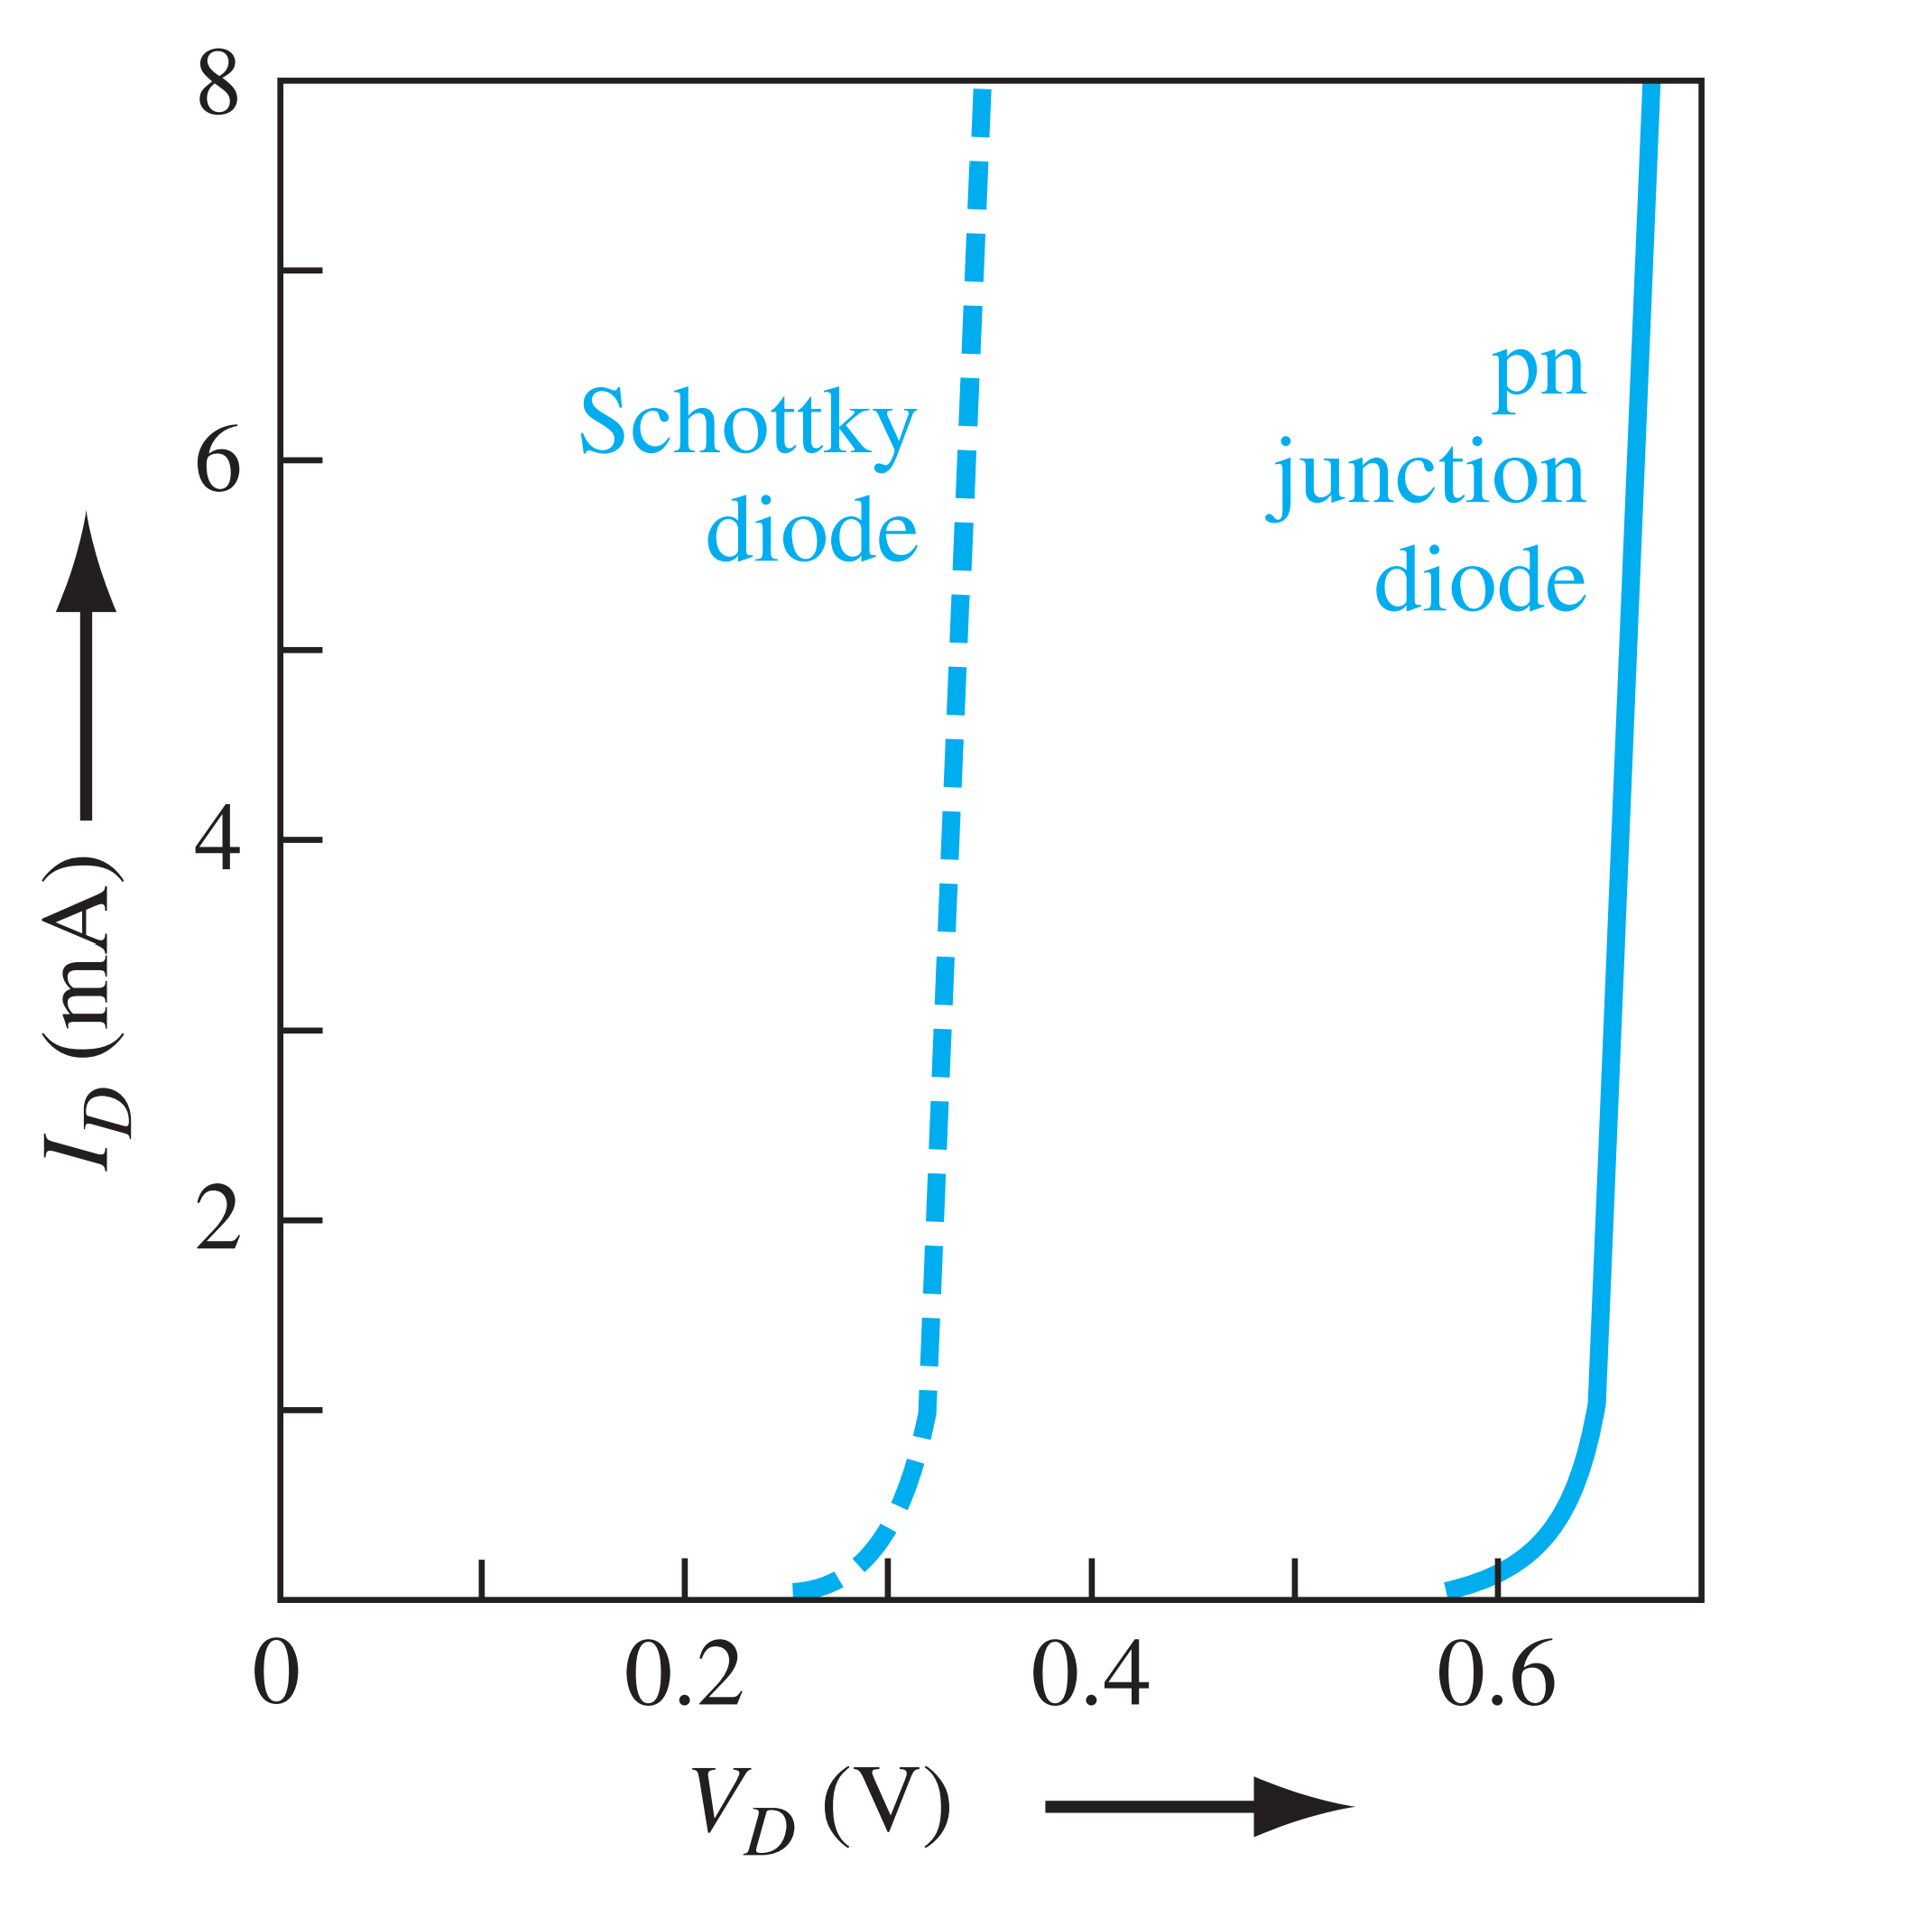
\includegraphics[width=8.5cm]{image/1.png}
\end{Figure}

除此之外,有趣的是,肖特基二极管和PN结二极管的反向电流实际上都不饱和
\begin{itemize}
    \item 对于肖特基二极管,原因是$J_{st}$会随着反偏电压的增大而增大。
    \item 对于PN结二极管,原因是反偏时另有产生电流$J_{gen}$会随反偏电压增大。
\end{itemize}

实际上,PN结二极管在反偏时占主导地位的是$J_{gen}$而不是$J_s$,但即便是$J_{gen}$也远小于肖特基二极管的$J_{sT}$,$J_{gen}$的典型值在$10^{-7}\si{A.cm^{-2}}$,$J_{sT}$的典型值在$10^{-5}\si{A.cm^{-2}}$。因此,即便是考虑了PN结的反偏产生电流$J_{gen}$,肖特基二极管的反偏电流仍远高于PN结二极管。

\subsubsection{关于频率响应的差异}
肖特基二极管和PN结二极管最大的区别在于,前者是多子器件,后者是少子器件,这就意味着,肖特基二极管并不存在扩散电容,因此可以被用于需要高频开关的场合。通常来说
\begin{itemize}
    \item 对于PN结二极管,其典型开关时间是纳秒级的。
    \item 对于肖特基二极管,其典型开关时间则可以达到皮秒级。
\end{itemize}

应当指出的是,尽管肖特基二极管看上去有很多优势,例如开启电压小和频率响应高等,但是这并不代表肖特基二极管可以完全取代PN结二极管。许多特性是有利有弊的,例如开启电压小就势必意味着更大的反偏电流,换言之,功耗高。最重要的是,工艺上形成PN结的成本和复杂性要远低于金半接触。基于这些原因,目前最为常用的二极管仍然是PN结二极管。

